\section{Our Design}
\label{sec:ourdesign}

After the headroom analysis, we come up with our design of dynamic hybrid prefetcher system. We name this as \emph{DHP}. The \emph{DHP} is built on the idea of \emph{Static Analysis}. For \emph{Static Analysis}, system takes performace files as input. In \emph{DHP}, these information should be recorded during the execution, using the storage structure explained in section \ref{sec:storestruct}. Then, apply heuristic to these stored information in order to make prefetch decisions.

  \subsection{Storage Structure}
  \label{sec:storestruct}
  \begin{figure}[ht!]
	   \centering
	   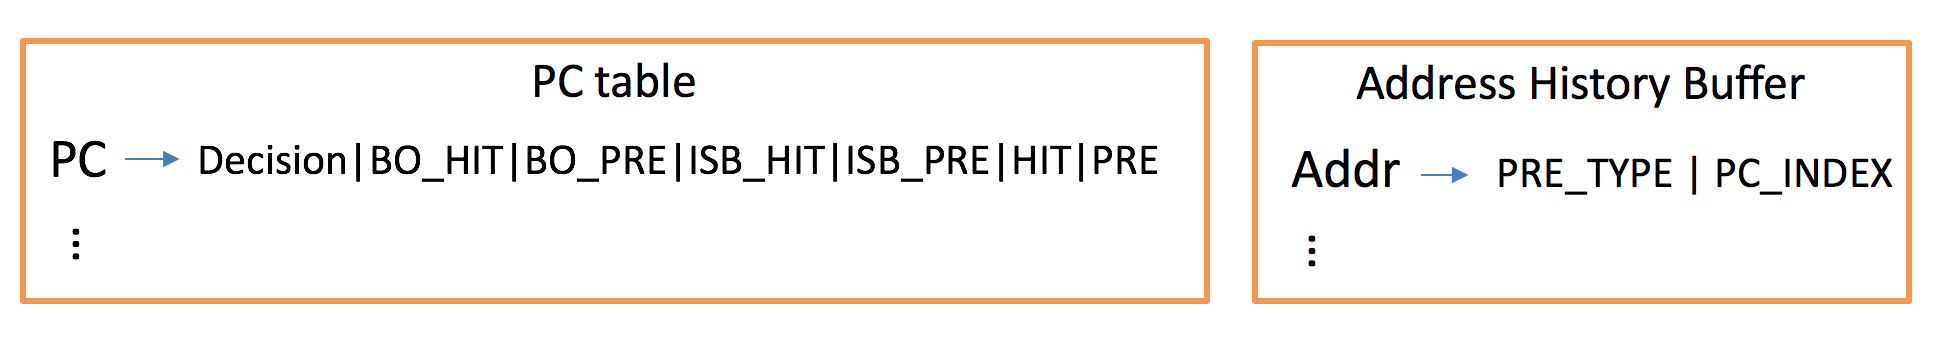
\includegraphics[width=1.0\textwidth]{images/storage_struct.png}
	   \caption{How one PC's and one Addr's information is organized}
	   \label{fig:storage_struct}
  \end{figure}

  The first structure is called \emph{PC Table}. The \emph{PC Table} stores the prefetch information of each prefetcher. Left part of Fig. \ref{fig:storage_struct} shows how one PC's information is recorded. \emph{BO/ISB HIT} and \emph{BO/ISB PRE} counts all the prefetches and hits issued by \emph{BO/ISB} using this PC. \emph{HIT} and \emph{PRE} count all the prefetches and hits made by this PC. Last but not least, \emph{Decision} represents the choice of this PC. Usually the number of load PC won't be too large, we choose 4096 as our PC table length.

  On the other hand, if there is a prefetch hit or the cache controller issues a prefetch, the corresponding address needs to know which PC actually prefetched it, so as to increment the correspoinding counter. \emph{PRE\_TYPE} represents which prefetcher issued the prefetch. It can be \emph{BOTH, ISB} or \emph{BO}. The \emph{PC\_Index} domain stores a back pointer pointing to the corresponding entry of the \emph{PC Table}. Actually one more slot is added to one Addr line, whose name is \emph{DANGER}. Sometimes different PC may prefetch the same address, the \emph{DANGER} value helps decide whether we need to change the PC index entry. Different from PC table, number of addresses visited in one benchmark is far more than the number of PC. Therefore, we design our address history buffer using 8*4096 entries. Old entries will be replaced if the address history buffer is full.

  \subsection{Design Overview}
  \label{sec:dynamicdesignoverview}
  \begin{figure}[ht!]
	   \centering
	   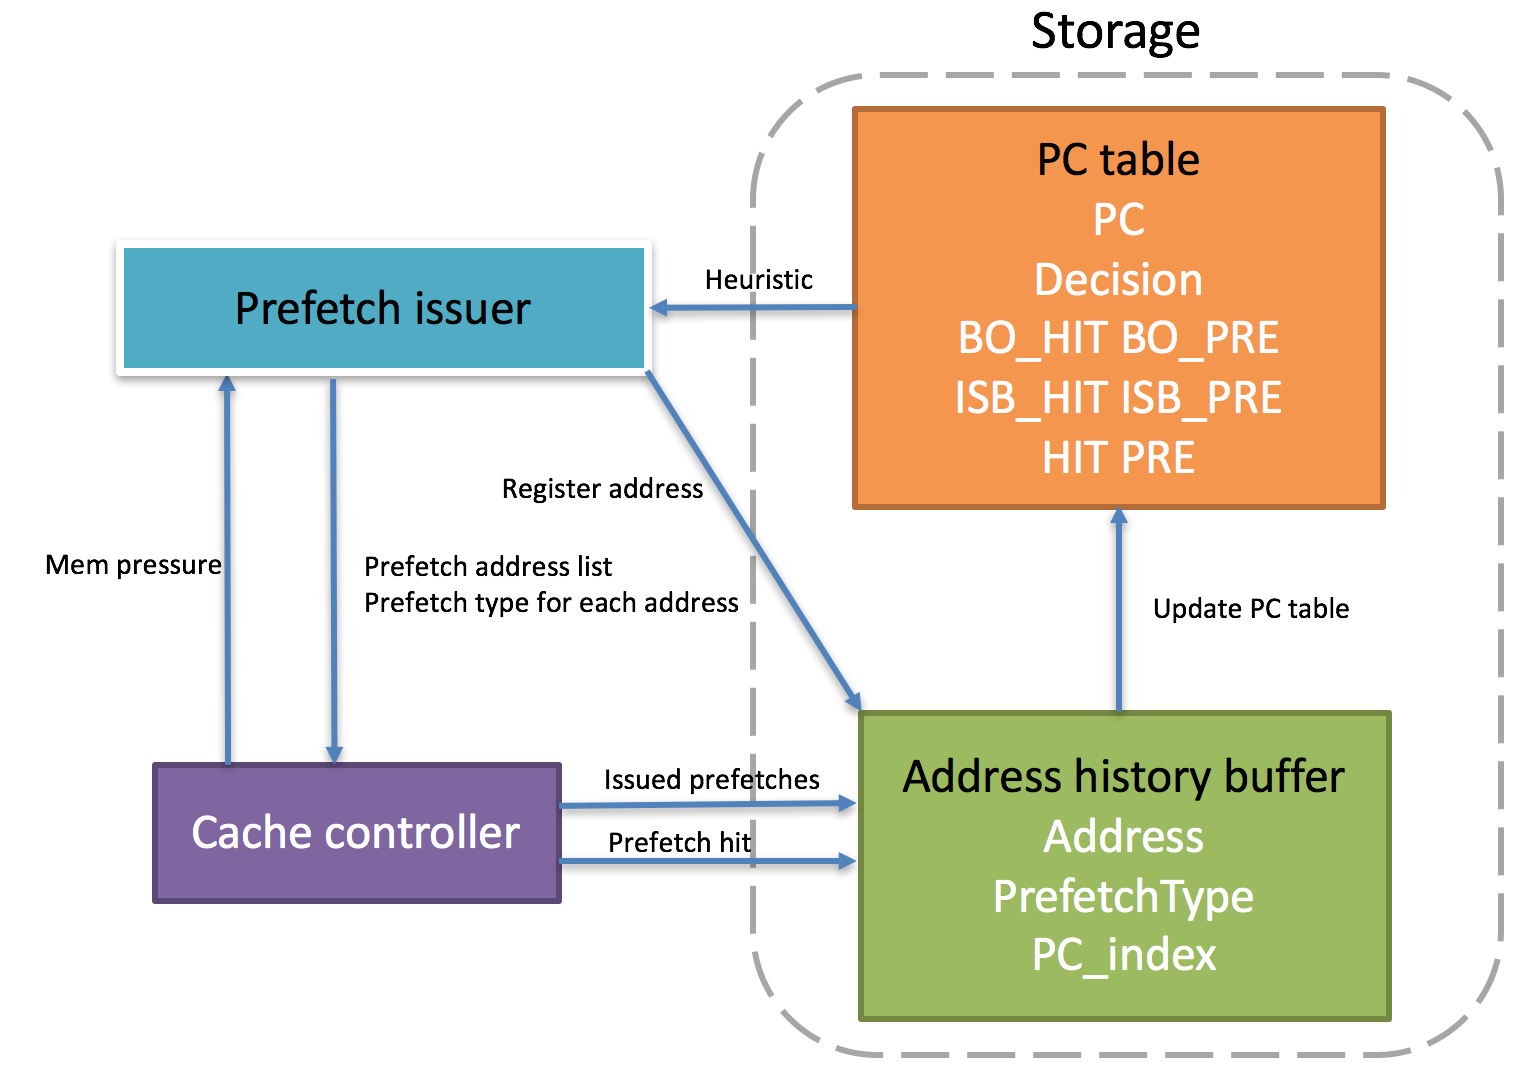
\includegraphics[width=0.8\textwidth]{images/dynamic_design.png}
	   \caption{Headroom speedup under different memory bandwidth}
	   \label{fig:dynamic_design}
  \end{figure}

  In Fig. \ref{fig:dynamic_design}, we show the our design of \emph{DHP}. The \emph{PC Table} and the \emph{Address History Buffer} serves the role of input files in \emph{Static Analysis} case. Here, I need to mention two important functions in the file \emph{cache\_cntlr.cc}. One is \emph{doPrefetch} and the other one is \emph{processShmemReqFromPrevCache}. The cache controller receive prefe 
